We present an overview of arithmetic operations in~$\mathbf{Q}_p$ 
and unramified extensions.  Much of the material is well-known in 
either the context of $p$-adic arithmetic itself, see e.g.\ 
Vercauteren~\citep[\S 12]{HEHCC2005} or integer arithmetic, 
see e.g.\ the survey by Bernstein~\citep{Bernstein2008}. 
The original contribution consists of the adaptation of an algorithm 
for computing the exponential function by Brent~\citep{Brent1976} 
to the case of $p$-adic arithmetic, and the derivation of a related 
algorithm for computing the logarithm function.  Moreover, this 
work is accompanied by an implementation in the open-source computational 
software {\sc FLINT}~\citep{FLINT}.

The sections on the $p$-adic exponential and logarithm functions 
are joint work with Fredrik Johansson, RISC, Austria.

\section{Data format}

We represent a non-zero $p$-adic number $x \in \mathbf{Q}_p$ in the form 
\begin{equation}
x = p^v u
\end{equation}
where $u, v \in \mathbf{Z}$ and $p \nmid u$.  When working to precision~$N$, 
it is sometimes useful to assume that $u \in [0,p^{N-v})$.

When working in the unique unramified extension of $\mathbf{Q}_p$ of 
degree~$d$, we which shall refer to as~$\mathbf{Q}_q$ where $q = p^d$ 
with ring of integers~$\mathbf{Z}_q$, we choose to represent this as 
\begin{equation}
\mathbf{Q}_q \cong \mathbf{Q}_p[X] / (f(X))
\end{equation}
where $f(x) \bmod p$ is an irreducible and separable polynomial.  We store 
$f(X)$ as a sparse polynomial and assume that its coefficients are 
reduced modulo~$p$.  If $f(X)$ has at most a constant number of non-zero 
terms, the reduction of a degree~$n$ polynomial modulo~$f(X)$ can be carried 
out in $\mathcal{O}(nd)$ additions and multiplications in $\mathbf{Q}_p$.  
With this set-up, a non-zero element~$g$ in~$\mathbf{Q}_q$ can be represented 
as 
\begin{equation}
g(X) = p^v h(X)
\end{equation}
where $v \in \mathbf{Z}$ and $h(X) \in \mathbf{Z}[X]$ is such that at least 
one coefficient of $h(X)$ is a $p$-adic unit and $\deg(h) < d$.  As before, 
it can be useful to assume that all coefficients of $h(X)$ are reduced 
modulo~$p^{N-v}$.

\begin{rem}
We could aim for a genuine base~$p$ representation, explicitly showing 
the $p$-adic digits in the form 
\begin{equation}
x = p^v (a_0 + a_1 p + a_2 p^2 + \dotsb) 
\end{equation}
with $a_i \in [0,p)$ for all $i$, or perhaps 
\begin{equation}
x = p^v (a_0 + a_1 p^k + a_2 p^{2k} + \dotsb)
\end{equation}
with $a_i \in [0,p^k)$ where $k$ is least such that $p^{k}$ fits into 
a machine word.
This data format would be beneficial to many algorithms.  But in practice, 
given the high quality and architecture specific details of implementations 
for arbitrary precision integer arithmetic in base~$2$, this approach does 
not seem favourable.
\end{rem}

\section{Review of complexity results and related definitions}

We let $\mathcal{O}(M(N))$ denote the complexity of multiplying two 
$N$-bit integers.  For example, the algorithm of 
Sch\"onhage--Strassen~\citep{SchoenhageStrassen1971}
allows us to take $M(N) = N \log N \log \log N$.  The same 
complexity can also be achieved for the division with remainder of 
a $2N$-bit integer by an $N$-bit integer.

As elements of $\mathbf{Z} / (p^N)$ are of bit size $N \log p$, 
multiplication of two numbers in $[0, p^N)$, with or without a subsequent 
reduction modulo $p^N$, has complexity $\mathcal{O}(M(N \log p))$.

Moreover, we let $\mathcal{O}(\mu(p,d,N))$ denote the 
complexity of multiplication in $\mathbf{Z}_q / (p^N)$.  This operation 
involves one multiplication of two degree $d-1$ polynomials in 
$\mathbf{Z}/(p^N)$ and one reduction of a degree $2d - 2$ polynomial 
in $\bigl( \mathbf{Z}/(p^N)[X] \bigr) / (f(X))$.  Using a Fast Fourier 
Transform based multiplication routine, the polynomial product requires 
$\mathcal{O}(d \log d)$ operations in $\mathbf{Z}/(p^N)$, hence has 
complexity $\mathcal{O}\bigl((d \log d) M(N \log p)\bigr)$.  The reduction 
modulo $f(X)$ also requires $\mathcal{O}(d \log d)$ ring operations 
in $\mathbf{Z}_p / (p^N)$ in general but only $\mathcal{O}(d)$ when 
$f(X)$ is \emph{sparse}, by which we mean that the number of non-zero 
coefficients of $f(X)$ is bounded independently of the parameters 
$p$, $d$, and $N$.  In either case, for later reference we can set 
$\mu = \mu(p,d,N) = (d \log d) M(N \log p)$.

In the remaining part of this chapter we make the assumption that 
the complexity of multiplying two $N$-bit integers satisfies 
$2 M(N) \leq M(2 N)$.  In particular, this allows us to show that 
for $k + 1$ multiplications of bit sizes $1, 2, \dotsc, 2^k$, 
\begin{equation}
M(1) + M(2) + \dotsb + M(2^k) \leq \bigl( 2^{-k} + 2^{-k+1} + \dotsb + 1 \bigr) M(2^k) \leq 2 M(2^k).
\end{equation}
This calculation shows that the complexity of Hensel lifting routines 
that we consider in the following sections is dominated by their last 
step at the greatest $p$-adic precision.

We also define $\omega$ to be the exponent of matrix multiplication, 
that is, such that the multiplication of two $n \times n$ matrices 
over a ring requires $\mathcal{O}(n^{\omega})$ ring operations.  The 
classical approach realises $\omega = 3$, the practical algorithm 
of Strassen~\citep{Strassen1969} achieves $\omega < 2.81$, and 
the still essentially best theoretical result by 
Coppersmith--Winograd~\citep{CoppersmithWinograd1990} shows 
that $\omega < 2.38$.

\section{Hensel lifting}

\begin{thm} \label{thm:Hensel1}
Let $g \in \mathbf{Z}_q[X]$ be a polynomial whose leading coefficient 
is a unit and suppose that $x_0 \in \mathbf{Z}_q$ is such that 
\begin{equation*}
\ord_p(g(x_0)) \geq m + n, \quad \ord_p(g'(x_0)) \leq m
\end{equation*}
for some $0 \leq m < n$.  Then there exists a unique $x \in \mathbf{Z}_q$ 
such that $g(x) = 0$ and $x \equiv x_0 \pmod{p^n}$.
\end{thm}

\begin{proof}
We construct a sequence $(x_k)$ such that 
\begin{align*}
\ord_p(g(x_k)) & \geq 2^k (n - m) + 2m, \\
\ord_p(g'(x_k)) & \leq m, \\
\ord_p(x_{k+1} - x_k) & \geq 2^k (n-m) + m, 
\end{align*}
where the choice of $x_{k+1}$ is unique given $x_k$, for $k \geq 0$.  
As the sequence $(x_k)$ is Cauchy, the result then follows taking 
$x = \lim_{k \to \infty} x_k$ and using the continuity of $g$ to 
establish $g(x) = 0$.

In order to satisfy the last condition, begin by writing 
$x_{k+1} = x_k + p^{2^k(n-m) + m} T$ and expand $g(x_{k+1})$ 
as a Taylor series about $x_k$, 
\begin{align*}
g(x_{k+1}) & = \sum_{j=0}^{\deg(g)} \frac{g^{(j)}(x_k)}{j!} p^{(2^k(n-m) + m) j} T^j \\
           & \equiv g(x_k) + g'(x_k) p^{2^k(n-m) + m} T \pmod{p^{2^{k+1}(n-m)+2m}}
\end{align*}
where the last line follows upon observing that $g^{(j)}(x_k) / j!$ 
is $p$-adically integral for all~$j$.  This forces the unique choice 
$x_{k+1} = x_k - g(x_k) / g'(x_k)$ modulo~${p^{2^{k+1}(n-m) + m}}$.
\end{proof}

\begin{rem}
In order to approximate the root of a polynomial to a desired 
precision~$N$, it is preferable to choose the sequence of 
precisions 
\begin{equation*}
e_{k} = N, e_{k-1} = \ceil{(e_k + m) / 2}, \dotsc, 
e_0 = \ceil{(e_1 + m) / 2} \leq n
\end{equation*}
as this choice minimises the computational cost in every step 
and in the dominating last step, in particular.
\end{rem}

\begin{thm} \label{thm:Hensel2}
Let $g \in \mathbf{Z}_q[X]$ be a polynomial whose leading coefficient 
is a unit and suppose that $x_0 \in \mathbf{Z}_q$ is such that 
\begin{equation*}
\ord_p(g(x_0)) \geq m + n, \quad \ord_p(g'(x_0)) \leq m
\end{equation*}
for some $0 \leq m < n$.  Moreover, let $x$ be the unique root of $g$ 
lifting $x_0$ and define the sequences
\begin{align*}
y_0 & = \bigl( g'(x_0) \bigr)^{-1}, \\
x_{k+1} & = x_k - g(x_k) y_k, \\
y_{k+1} & = y_k \bigl( 2 - y_k g'(x_{k+1}) \bigr),
\end{align*}
where $x_k$, $y_k$ are computed to $p$-adic precision $2^k (n-m) + m$.
Then $x_k$ agrees with $x$ modulo~$p^{2^k (n - m) + m}$.
\end{thm}

\begin{rem}
The above theorem leads to an algorithm running two Hensel lifting 
procedures in parallel, which is favourable to the approach suggested 
by the expression $x_{k+1} = x_k - g(x_k) / g'(x_k)$ in 
Theorem~\ref{thm:Hensel1}, which leads to a nested lifting routine to 
compute the inverse of $g'(x_k)$ from scratch at each step.
\end{rem}

\section{Addition, subtraction, negation}

In order to add $x_0, x_1 \in \mathbf{Q}_q$ to precision~$N$, 
we compute 
\begin{equation}
x_0 + x_1 = p^{v_0} (u_0 + p^{v_1 - v_0} u_1)
\end{equation}
where we assume $v_0 \leq v_1$.  Note that the second factor may 
only be divisible by~$p$ if $v_0 = v_1$.  Moreover, the second factor 
will have to be reduced modulo $p^{N - v_0}$ using a division 
routine.  We can improve on this if we add the assumption that 
the input is reduced modulo $p^N$, in which case we observe that 
there the reduction can be facilitated by subtracting at most 
one multiple of~$p^{N-v_0}$.

\section{Multiplication}

Given $x_0, x_1 \in \mathbf{Q}_q$, we can compute their product 
to precision~$N$ via 
\begin{equation}
x_0 x_1 = p^{v_0 + v_1} u_0 u_1,
\end{equation}
reducing the product of units $u_0 u_1$ modulo $p^{N - v_0 - v_1}$.

\section{Inversion}

Suppose that we want to compute the inverse of $x = p^v u \in \mathbf{Q}_q$ 
to precision~$N$.  Note that the inverse has valuation $-v$ and hence 
whenever $-v \geq N$ we return zero.  Otherwise, our aim is to compute 
the inverse of $u \in \mathbf{Z}_q^{\times}$ to precision~$N+v$.

In order to compute the inverse of $u \in \mathbf{Z}_q^{\times}$, we 
apply Hensel lifting on the polynomial $g(X) = 1 - u X$, leading to 
the iteration
\begin{equation} \label{eq:padic-inverse}
\begin{split}
x_{k + 1} & = x_k - x_k (x_k u - 1), \\
          & = x_k (2 - x_k u), \\
          & = 2 x_k - u x_k^2
\end{split}
\end{equation}
starting from an approximation modulo~$p$.

Note that we provide various expressions for $x_{k+1}$ in 
Equation~\eqref{eq:padic-inverse}.  Roughly speaking, and ignoring 
the logarithmic dependence on~$p$, the second expression consists of 
one $2^k$-by-$2^{k+1}$ bit product and one $2^k$-by-$(3 \times 2^k)$ bit 
product whereas the third expression consists of one $2^k$-by-$2^k$ bit 
product and one $2^{k+1}$-by-$2^{k+1}$ bit product.

Inverses over finite fields can be computed efficiently by 
extended greatest common divisor algorithms, for example, using 
Euclid's algorithm or the asymptotically fast Half-GCD 
algorithm~\citep{ThullYap1990}, which requires 
$\mathcal{O}\bigl(n (\log n)^2\bigr)$ operations in $\mathbf{F}_p$ 
for two input polynomials in $\mathbf{F}_p[X]$ of degree~$\mathcal{O}(n)$.  
An improvement to the general method can be made by computing only one 
cofactor, that is, when computing $s, t$ such that $1 = \gcd(a,b) = sa + tb$ 
we in fact only require one of the two cofactors $s, t$.

Following this procedure, the complexity of inverting an element of 
$\mathbf{Z}_q^{\times}$ to precision~$N$ is given by 
$\mathcal{O}\bigl( d (\log d)^2 M(\log p) + \mu \bigr)$.

\section{Inverse square root}

The method of computing $p$-adic inverse square roots turns out 
to be interesting because it will be used as a precursor in computing 
$p$-adic square roots.

Given a non-zero $x = p^v u \in \mathbf{Q}_q$, the task is to compute 
one of its inverse square roots $p^{-v/2} u^{-1/2}$.  Necessarily, 
we require that $v$ is even and $u$ a square in~$\mathbf{Z}_q^{\times}$.

The computation then reduces to computing $p$-adic inverse square 
roots of $u \in \mathbf{Z}_q^{\times}$, which can be carried out 
using a Hensel lifting approach on $g(X) = 1 - u X^2$.  This leads 
to the almost division-free iteration
\begin{equation}
\begin{split}
x_{k+1} & = x_k + (1 - u x_k^2) / (2 u x_k) \\
        & = x_k + x_k (1 - u x_k^2) / 2
\end{split}
\end{equation}
In the notation of Theorem~\ref{thm:Hensel1}, this means that when 
$p > 2$ is an odd prime we can take $m = 0$, $n = 1$, but when $p = 2$ 
the division by~$2$ in the above formula forces us to account for 
the precision loss, taking $m = 1$, $n = 2$.

When $p = 2$, we can obtain an initial approximation as follows. 
Let $s = (u \bmod 2)^{-1/2} \pmod{2}$.  If there exists a solution~$t$ 
to $t^2 + s t \equiv (1/u - s^2) / 4 \pmod{2}$ then $x_0 = s + 2 t$ 
is an approximate inverse square root of $u$ to precision~$2$, 
otherwise $u$ is not a square modulo~$8$ and hence not a square 
in~$\mathbf{Z}_q^{\times}$.  When $p > 2$ is an odd prime, we can 
take the inverse square root modulo~$p$ as our initial approximation.
However, the topic of computing square roots in finite fields is outside 
the scope of this discussion.  We refer the reader to standard 
results in finite field arithmetic, e.g.\ as presented in 
Bach--Shallit~\mbox{\citep[\S 7]{Bac96}}.

We observe that this iteration does indeed not require computationally 
intensive $p$-adic inversions.  When $p$ is odd, either the numerator 
is divisible by~$2$ as an integer, or we can add an appropriate (odd) 
power of~$p$ to this, yielding an even integer representative of the 
same value.  The division by~$2$ is then simply a bitshift.  When $p = 2$, 
the result on Hensel lifting in Theorem~\ref{thm:Hensel1} guarantees that 
the numerator is always divisible by~$2$ and the loss of precision is 
accounted for in the sequence of precisions.

We now discuss the complexity of this operation.  The initial step 
modulo~$p$ consists of an inversion and a square root in $\mathbf{F}_q$. 
The first of these can be achieved using the Half-GCD algorithm 
in $\mathcal{O}\bigl(d (\log d)^2\bigr)$ operations in $\mathbf{F}_p$.  
The second problem is easy in practice but much harder in theory.  According 
to Bach--Shallit~\citep[\S 7, Exercise~34]{Bac96}, 
it can be solved in $\mathcal{O}\bigl((d + \log p) (\log p)^2\bigr)$ 
bit operations using a probabilistic algorithm.  The theoretically 
difficult part is the determination of a non-square element 
in~$\mathbf{F}_q^{\times}$ when $q$ is odd, but the algorithm can be 
made deterministic assuming the Extended Riemann Hypothesis.  In terms 
of the dependency on~$N$, the main contribution comes from the 
deterministic Hensel lifting procedure, which as in the case of 
inversion has complexity~$\mathcal{O}(\mu)$.  The overall complexity 
is given by the sum of the above three estimates since none dominates 
another as the parameters $p$, $d$, and $N$ vary independently.

\section{Square root}

We observe that a non-zero $x = p^v u \in \mathbf{Q}_q$ has a square 
root if and only if $v$ is even and $u \in \mathbf{Z}_q^{\times}$ is 
a square.  Thus, for the remaining part of the discussion we may 
assume that $u \in \mathbf{Z}_q^{\times}$ is a square.

In order to compute $\sqrt{u}$ modulo~$p^N$, we can use the previous method 
for computing the inverse square root to precision~$N$ and then multiply 
the result by~$u$.  This approach is favourable in pracice as the Hensel 
lifting iteration is more efficient for inverse square roots than for 
square roots.
As noted by Karp and Markstein~\citep{KarpMarkstein1997}, this algorithm 
can be improved by replacing the final iteration in the Hensel lifting 
procedure for the inverse square root by 
\begin{align}
t       & = u x_k \pmod{p^{N'}} \\
x_{k+1} & = t + x_k (u - t^2) / 2 \pmod{p^N}
\end{align}
where $N'$ is the precision in the penultimate step, and omitting the 
subsequent multiplication by~$u$ mentioned above.

The approach described above clearly has the same complexity as the 
algorithm for the inverse square root problem. 

\section{Teichm\"uller lift}

Recall that $\mathbf{Q}_q$ contains exactly $(q-1)$~elements that are 
$(q-1)$th roots of unity, one above each non-zero element of the residue 
field $\mathbf{F}_q$.  The Teichm\"uller lift of an element 
$u \in \mathbf{F}_q^{\times}$ is defined to be the unique lift to a 
$(q-1)$th root of unity 
in~$\mathbf{Q}_q$.

In order to compute the Teichm\"uller lift of $u \in \mathbf{F}_q^{\times}$, 
we apply Hensel lifting on $g(X) = X^q - X$, starting with $x_0 = u$ and 
noting that $\ord_p(g'(x_0)) = 0$. 

As a noticeable practical improvement, we observe that the denominators 
$g'(x_k) = q x_k^{q-1} - 1$ converge to $q-1$, which is defined over 
$\mathbf{Z}_p$ already, in a way such that $\ord_p\bigl(g'(x_k) - (q-1)\bigr)$ 
is non-decreasing.  Thus, we can replace the Hensel lifting iteration by 
\begin{equation}
x_{k+1} = x_k - (q-1)^{-1} (x_k^q - x_k), 
\end{equation}
also noting that $(q-1)^{-1}$ only has to be computed to the precision 
of the previous step.

The complexity of this approach is dominated by the evaluations 
of $g(x_k) = x_k^q - x_k$ to the precisions $2, \dotsc, \ceil{N/2}, N$ 
during the Hensel lifting procedure.  Using binary exponentiation, 
computing the power $x_k^q$ requires $\mathcal{O}(\log q)$ operations 
in $\mathbf{Z}_q$ to the appropriate $p$-adic precision at each step. 
Thus, the complexity is given by $\mathcal{O}\bigl((\log q) \mu\bigr)$.

\section{Frobenius}

Let $\Sigma \in \Gal(\mathbf{Q}_q/\mathbf{Q}_p) \cong \Gal(\mathbf{F}_q/\mathbf{F}_p)$ 
be the lift of $\sigma \colon \mathbf{F}_q \mapsto \mathbf{F}_q, x \mapsto x^p$. 
For any $x \in \mathbf{Q}_q$ and $k \in \mathbf{Z}$, we aim to compute $\Sigma^k x$ 
modulo $p^N$, noting that $\Sigma$ has order~$d$.  As such, we may assume that~$k$ 
is reduced modulo~$d$, and in fact that $0 < k < d$ as $\Sigma^0$ is the identity map.
Moreover, as $\Sigma$ is a $\mathbf{Q}_p$-linear map, we may assume that 
$x = \sum_{i=0}^{d-1} a_i X^i$ is a unit in $\mathbf{Z}_q$.  

First, we can compute $\Sigma^k X$ using Hensel lifting on $f(X)$, 
starting from $x_0 = X^{p^k}$ in $\mathbf{F}_p[X] / (f(X))$.  We note 
that there is no precision loss during the Hensel lifting procedure;  
in the notation of Theorem~\ref{thm:Hensel1}, we can take $m = 0$, $n = 1$. 
This is because $f \bmod p$ is separable and hence $f'(x_0) \bmod p$ is 
non-zero.  At each step, the Hensel lifting routine involves the computations 
of $f(x_k)$ and $f'(x_k)$, which are polynomial compositions modulo~$f(X)$ 
and a power of~$p$.  We discuss the general case of modular compositions 
further below, but note here that when $f(X)$ is sparse the naive approach 
to composition requires only $\mathcal{O}\bigl((\log d) \mu\bigr)$.

Finally, we can compute $\Sigma^k x$ via 
\begin{equation}
\Sigma^k x = 
    \Sigma^k \bigl( \sum_{i=0}^{d-1} a_i X^i \bigr) = 
    \sum_{i=0}^{d-1} a_i (\Sigma^k X)^i, 
\end{equation}
which entails a polynomial composition modulo~$f(X)$ and~$p^N$.

In a first approach, we might use Horner's method to carry out the 
composition, which requires about $d$~multiplications in $\mathbf{Z}_q$, 
yielding a complexity of $\mathcal{O}(d \mu)$.  

However, we can use the rectangular splitting approach due to 
Paterson--Stockmeyer~\citep{PatersonStockmeyer1973} instead, based 
on the expression 
\begin{equation}
\Sigma^k x = \sum_{i=0}^{\floor{d/B}-1} \Bigl( \sum_{j=0}^{B-1} a_{Bi + j} (\Sigma^k X)^j  \Bigr) (\Sigma ^k X)^{Bi},
\end{equation}
where $B = \floor{\sqrt{d}}$ and we define $a_{Bi + j} = 0$ whenever 
$Bi + j \geq d$, note that in the last iteration the inner sum generally 
has fewer than $B$ terms.  From an algorithmic point of view, it is 
important that this allows us to precompute $\Sigma^k(X)^i$ for 
$i = 0, \dotsc, B$.  Thus, this approach only requires about 
\mbox{$2 \sqrt{d}$}~multiplications in $\mathbf{Z}_q$ but additional space 
for about $d^{3/2}$~elements of $\mathbf{Z}/(p^N)$.  As there are another 
$d$~scalar multiplications of elements of~$\mathbf{Z}_q$ by elements of 
$\mathbf{Z}_p$, the complexity of this polynomial composition 
is given by $\mathcal{O}\bigl(\sqrt{d} \mu + d^2 M(N \log p)\bigr)$, which 
is $\mathcal{O}\bigl(d^2 M(N \log p)\bigr)$.  Thus, the asymptotic 
improvement in~$d$ when compared to Horner's method 
only consist of removed logarithmic factors, however, in practive the smaller 
number of $\mathbf{Z}_q$-multiplications is important.

This can be improved asymptotically by employing the modular composition 
algorithm of Brent--Kung~\citep{BrentKung1978}, which requires only 
$\mathcal{O}(n^{(\omega+1)/2})$ ring operations when all three input 
polynomials have degrees $\mathcal{O}(n)$, where $\omega$ is the exponent 
of matrix multiplication.  Here, the ring in question in $\mathbf{Z}/(p^N)$ 
and the polynomials have degree at most~$d$, hence we obtain the bit 
complexity estimate $\mathcal{O}(d^{(\omega + 1)/2} M(N \log p)\bigr)$.

We now discuss the overall complexity of the computation of $\Sigma^k x$.
Using a method for binary exponentiation, computing \mbox{$x_0 = X^{p^k}$} 
requires about $k \log p$~products in~$\mathbf{F}_p[X] / (f(X))$ and hence 
has complexity $\mathcal{O}\bigl((d \log p) \mu(p,d,1)\bigr)$.  The Hensel 
lifting routine is dominated by its last step, which involves evaluating 
$f(x_k)$ and $f'(x_k)$ in $\mathbf{Z}_q$ to precision~$N$.  This in turn 
consists of two modular compositions.  As described above, the final step 
is another modular composition.  Thus, the overall complexity is given by 
$\mathcal{O}\bigl( (d \log p) \mu(p,d,1) 
+ d^{(\omega + 1)/2} M(N \log p) \bigr)$.

\section{Trace}

The image of $x \in \mathbf{Q}_q$ under the trace function 
$\Trace_{\mathbf{Q}_q/\mathbf{Q}_p} \colon \mathbf{Q}_q \to \mathbf{Q}_p$ 
is defined as the sum of the Galois conjugates of~$x$.  Equivalently, 
it is defined as the trace of the $\mathbf{Q}_p$-linear map on 
$\mathbf{Q}_q$ given by multiplication by~$x$.  As the trace map 
itself is $\mathbf{Q}_p$-linear, we may now assume that 
$x \in \mathbf{Z}_q^{\times}$.

There are two efficient ways to compute this:

First, we can compute this from the definition of $\Trace(x)$ as the trace 
of the multiplication-by-$x$ map by reducing $x X^i$ modulo $f(X)$ and forming 
the sum of the $X^i$-coordinates, for $i = 0, \dotsc, d - 1$.

Recalling that the reduction of a degree~$2d-2$ polynomial modulo 
$f(X)$ in $\mathbf{Z}/(p^N)$ requires time~$\mathcal{O}(\mu)$, 
it is clear that this approach takes time~$\mathcal{O}(d \mu)$. 
When we assume that $f(X)$ is sparse, this decreases to 
$\mathcal{O}\bigl(d^2 M(N \log p)\bigr)$.

Alternatively, we can observe that on writing $x = \sum_{i=0}^{d-1} a_i X^i$ 
we have $\Trace(x) = \sum_{i=0}^{d-1} a_i \Trace(X^i)$ and then use the 
Newton--Girard formulae,
\begin{equation} \label{eq:03-03-trace}
\Trace(X^i) + \sum_{j=1}^{i-1} \Trace(X^{i-j}) f_{d-j} + i f_{d-i} = 0 \pmod{p^N}, 
\end{equation}
for $i = 1, \dotsc, d-1$, where $f(X) = \sum_{i=0}^{d-1} f_i X^i$.  
We also note that $\Trace(X^0) = \Trace(I) = d$.  This approach visibly 
requires time $\mathcal{O}\bigl(d^2 M(N \log p)\bigr)$ in general.  When 
$f(X)$ is sparse, this further decreases to $\mathcal{O}(d M(N \log p))$ as 
the sum in Equation~\eqref{eq:03-03-trace} has a bounded number of 
non-zero terms.

\section{Norm}

The image of $x \in \mathbf{Q}_q$ under the norm function 
$\Norm_{\mathbf{Q}_q/\mathbf{Q}_p} \colon \mathbf{Q}_q \to \mathbf{Q}_p$ 
is defined as the product of the Galois conjugates of~$x$.  Thus, for 
$x \in \mathbf{Q}_q$ and $\lambda \in \mathbf{Q}_p$, we have that 
$\Norm(\lambda x) = \lambda^d \Norm(x)$ and we may hence assume that 
$x \in \mathbf{Z}_q^{\times}$.  Since 
$\Gal(\mathbf{Q}_q/\mathbf{Q}_p) = \langle \Sigma \rangle$ is cyclic 
of order~$d$, we find that, letting $a(X) \in \mathbf{Z}_p[X]$ denote 
the same polynomial as $x = \sum_{i=0}^{d-1} a_i X^i$, 
\begin{equation}
\begin{split}
\Norm_{\mathbf{Q}_q/\mathbf{Q}_p} (x) & = \prod_{i=0}^{d-1} \Sigma^i (x) \\
                                      & = \prod_{i=0}^{d-1} a(\Sigma^i(X)) \\
                                      & = \ell(f)^{- \deg(a)} \Res(f(X), a(X)).
\end{split}
\end{equation}
where $\ell(f)$ denotes the leading coefficient of $f(X)$.  

The resultant of $f(X)$ and $a(X)$ can be defined as the 
determinant of the Sylvester matrix~\citep[Lemma~3.3.4]{Coh93}, which is a 
square matrix over~$\mathbf{Z} / (p^N)$ with $\deg(f) + \deg(a) \leq 2d - 1$ 
columns. In order to avoid precision loss, this can be computed with the 
division-free determinant algorithm of Kaltofen~\citep{Kaltofen1992}, which 
requires $\mathcal{O}(d^{\omega/2 + 2} \log d \log \log d)$ ring operations 
in~$\mathbf{Z} / (p^N)$ where $\omega$ is the exponent for matrix multiplication.
Thus, the bit complexity of this computation can be given by 
$\mathcal{O}\bigl((d^{\omega/2 + 2} \log d \log \log d) M(N \log p)\bigr)$.

We note, however, that we have only implemented the simpler division-free 
determinant algorithm of Seifullin~\citep[Algorithm~4.2]{Seifullin2002}, 
which requires $\mathcal{O}(n^4)$ ring operations to compute the 
determinant of an $n \times n$~matrix.  This leads to a bit complexity 
estimate for the norm computation of $\mathcal{O}\bigl(d^4 M(N \log p)\bigr)$.

Whenever $x \in \mathbf{Z}_q^{\times}$ satisfies $\ord_p(x-1) > (p-1)^{-1}$ 
we can typically improve on this significantly, computing the norm via
\begin{equation}
\Norm_{\mathbf{Q}_q / \mathbf{Q}_p} (x) 
= \exp \bigl(\Trace_{\mathbf{Q}_q / \mathbf{Q}_p} (\log (x))\bigr).
\end{equation}
We omit a detailed analysis of the complexity of this approach, but note 
that together with the asymptotically fast algorithm for the logarithm 
function it behaves quasi-linearly in $d$ and $N$ when $f(X)$ is sparse.

\section{Exponential}

\subsection{Definition}

For $x \in \mathbf{Z}_q$ with $\ord_p(x) \geq 2$ or $\ord_p(x) \geq 1$ 
as $p=2$ or $p > 2$, respectively, the $p$-adic exponential functions is 
defined via 
\begin{equation}
\exp(x) = \sum_{i = 0}^{\infty} \frac{x^i}{i!}.
\end{equation}
In order to compute $\exp(x)$ modulo $p^N$, using that for positive 
integers~$z$, we have
\begin{equation}
\ord_p(z!) = \frac{z - s_p(z)}{p - 1} \leq \frac{z}{p - 1}
\end{equation}
where $s_p(-)$ denote the sum of $p$-adic digits, we are led to compute 
the truncated series 
\begin{equation} \label{eq:exp-trunc}
\exp(x) = \sum_{i = 0}^{n-1} \frac{x^i}{i!}
\end{equation}
where $n = \ceilbig{\bigl( (p-1)N - 1 \bigr) / \bigl( (p-1)v - 1 \bigr)}$ 
with $v = \ord_p(x)$.

Note that we require $\mathcal{O}(N)$ terms of the sum, 
and that when computing these iteratively for $i = 0, \dotsc, n-1$ 
each update step of the summand amounts to multiplication by $x / i$, 
which consists of an inversion in $\mathbf{Z}_p$, a scalar multiplication 
in $\mathbf{Z}_q$, and a product in $\mathbf{Z}_q$.  Altogether, this 
yields the complexity estimate $\mathcal{O}(N \mu)$, which is quasi-quadratic 
in~$N$.

\subsection{Rectangular splitting}

The rectangular splitting algorithm due to Patterson and 
Stockmeyer~\citep{PatersonStockmeyer1973} applied to the 
case of the $p$-adic exponential evaluates the truncated 
series~\eqref{eq:exp-trunc} using the expression 
\begin{align}
\exp(x) & = \sum_{j=0}^{\ceil{n/B} - 1} 
            \biggl( \sum_{i=0}^{B-1} \frac{x^i}{(Bj + i)!} \biggr) x^{Bj} \\
        & = \sum_{j=0}^{\ceil{n/B} - 1} 
            \frac{1}{(B (j+1) - 1)!} \biggl( \sum_{i=0}^{B-1} \frac{(B (j+1) - 1)!}{(Bj + i)!} x^i \biggr) x^{Bj} \\
        & = \frac{1}{(n-1)!} \sum_{j=0}^{\ceil{n/B} - 1} 
            \frac{(n-1)!}{(B (j+1) - 1)!} \biggl( \sum_{i=0}^{B-1} \frac{(B (j+1) - 1)!}{(Bj + i)!} x^i \biggr) x^{Bj}
\end{align}
where $B = \floorts{\sqrt{n}}$ and we omit the detail that 
in the last iteration in inner sum generally has fewer than 
$B$~terms.

There are three noticeable advantages to this approach.  Firstly, it 
reduces the number of $p$-adic inversions as now the division in the 
inner sum is an exact integer division.  Secondly, the scalar factors 
in the inner sum $(B j + i + 1) \dotsm (B j + B - 1)$ are only of size 
$\mathcal{O}(\sqrt{n} \log n)$.  Thirdly, in the case when $q > p$, 
this approach reduces the number of multiplication in~$\mathbf{Q}_q$.

We present the details in Algorithm~\ref{alg:exp-rectangular}.  In order 
to conclude that this approach does not lead to an asymptotic improvement 
in~$N$, we observe that the inner loop contains a scalar product where the 
scalar has bit size $\mathcal{O}(\sqrt{N} \log N)$ and the 
vector has $d$~coefficients each of bit size $\mathcal{O}(N \log p)$.  
As this statement is executed about~$N$ times, the time complexity is still 
quasi-quadratic in~$N$.

\begin{algorithm}
\caption{Computing the exponential via rectangular splitting}
\label{alg:exp-rectangular}
\begin{algorithmic}
\vspace{1mm}
\Require Integer $x \in [1,p^N)$ with $v = \ord_p(x) > (p-1)^{-1}$,
\Ensure  $\exp(x) \bmod{p^N}$.
\Procedure{ExpRectangular}{$x, p, N$}
\State $n \gets \ceil{((p-1)N - 1) / ((p-1)v - 1)}$
\If{$n \leq 3$}
\Return $\sum_{i=0}^{n-1} x^i / i! \bmod{p^N}$
\Else
\State $k \gets \floor{(n-2)/(p-1)}$
\State $B \gets \floor{\sqrt{n}}$
\For{$i = 0 \text{\bf{ to }} B$}
\State $x^{(i)} \gets x^i \bmod {p^{N + k}}$
\EndFor
\State $S \gets 0$
\State $f \gets 1$
\For{$i = \ceil{n/B} - 1 \text{\bf{ to }} 0 \text{\bf{ by }} -1$}
\State $\ell \gets i B$
\State $s \gets 0$
\State $c \gets 1$
\For{$h = \min\{n-1, \ell + B - 1\} \text{\bf{ to }} \ell \text{\bf{ by }} -1$}
\State $s \gets s + c x^{(h-\ell)}$
\If {$h \neq 0$}
\State $c \gets h c$
\EndIf
\EndFor
\State $S \gets s f + S x^{(B)} \bmod{p^{N + k}}$
\State $f \gets c f$
\EndFor
\Return $f^{-1} S \bmod {p^N}$
\EndIf
\EndProcedure
\end{algorithmic}
\end{algorithm}

\subsection{Binary splitting}

In this section, we describe Brent's binary splitting, or bit-burst 
algorithm~\citep{Brent1976} for computing the exponential function, 
adapted to the $p$-adic case.  In order to simplify the exposition, 
we restrict ourselves to the case of $\mathbf{Q}_p$ but note that 
it is possible to obtain the same asymptotic results in terms of 
their dependency on~$N$ in the case of $\mathbf{Q}_q$.

\subsubsection{Exponential, exact rational}

Algorithm~\ref{alg:exp-bsplit} computes the sum 
\begin{equation}
(a-1)! x^{1-a} \sum_{i=a}^{b-1} \frac{x^i}{i!}
\end{equation}
as an exact rational number.  This expression is chosen in such a way 
as to allow for a recursive computation of the exponential series. 
Visibly, we can invoke this routine with $a = 1$, $b = n$ in order 
to compute $\sum_{i=1}^{n-1} x^i / i!$.

\begin{algorithm}
\caption{Computing the exponential as an exact rational}
\label{alg:exp-bsplit}
\begin{algorithmic}
\vspace{1mm}
\Require Integer~$x$, integers $1 \leq a < b$.
\Ensure  $P = x^{b-a}$, $Q = (b-1)! / (a-1)!$, $T = (b-1)! x^{1-a} \sum_{i=a}^{b-1} x^i / i!$.
\Procedure{ExpBSplit}{$P, Q, T, x, a, b$}
\If{$b - a = 1$}
\State $(P, Q, T) \gets (x, a, x)$
\ElsIf{$b - a = 2$}
\State $(P, Q, T) \gets (x^2, a (a + 1), x (a + 1) + x^2)$
\Else
\State $m \gets \floor{(a + b) / 2}$
\State \Call{ExpBSplit}{$P_0, Q_0, T_0, x, a, m$}
\State \Call{ExpBSplit}{$P_1, Q_1, T_1, x, m, b$}
\State $P \gets P_0 P_1$
\State $Q \gets Q_0 Q_1$
\State $T \gets T_0 Q_1 + P_0 T_1$
\EndIf
\EndProcedure
\end{algorithmic}
\end{algorithm}

We now provide a sketch of the complexity analysis, assuming for 
simplicity that $a = 1$ and $b = n = 2^k + 1$.  Let us label the various 
levels in the recursive procedure $0, 1, \dotsc, k$ with $0$ and $k$ 
denoting the base cases and the top level, respectively.  We begin 
by estimating the size of the return values $P, Q, T$ at each level~$i$. 
Initially, when $i = 0$, $P$, and $T$ are of the same size as $x$ 
and $Q$ is at most $n$.  At level~$i$, $P$ is equal to $x^{2^i}$ 
and hence of size $2^i \log x$ bits.  $Q$ is the product of 
$2^i$ numbers at most $n$ and hence of size at most $2^i \log n$. 
Finally, from the expression $T \gets T_0 Q_1 + P_0 T_1$, we see 
that at level~$i$ the size of $T$ is at most 
$2^i \max \{\log n, \log x\} + i$. 
We now count the number of operations at each level.  At level~$0$ 
we only set $P$, $Q$, and $T$, and this is carried out $2^k$ times. 
At levels $i = 1, \dotsc, k$, we carry out the following operations 
$2^{k-i}$ times:  two products with factors of size at most 
$2^{i-1} \max\{ \log n, \log x \} + (i-1)$ bits, one product with 
factors of size $2^{i-1} \log x$, and one product with factors of 
size at most $2^{i-1} \log n$ bits.  Here, we ignore the computation 
$m \gets \floor{(a+b)/2}$ and the sum in $T \gets T_0 Q_1 + P_0 T_1$. 
Thus, we can form the estimate,
\begin{align*}
\sum_{i=1}^k 2^{k-i} M \bigl( 2^{i-1} \max\{ \log n, \log x \} 
                             + (i - 1)\bigr) 
& \leq \sum_{i=1}^k 2^{k-i} M \bigl( 2^{i} \max\{ \log n, \log x \} \bigr) \\
& \leq \sum_{i=1}^k 2^{k-i} 2^{-k+i} M \bigl( 2^{k} \max\{ \log n, \log x \} \bigr) \\
& \leq (\log n) M \bigl( n \max\{ \log n, \log x \} \bigr)
\end{align*}
and conclude that the complexity is given by 
$\mathcal{O}\bigl((\log n) M(n \max\{ \log n, \log x\})\bigr)$.

\subsubsection{Main part}

We now describe how to evaluate the truncated series 
$\sum_{i=0}^{n-1} x^i / i! \bmod{p^N}$ where we may assume 
that $0 < x < p^N$.  First, write 
\begin{equation}
x = \sum_{i=1}^{\ceil{\log_p N}} x_i
\end{equation}
with $0 \leq x_i < p^{2^i}$ and $\ord_p(x_i) \geq 2^{i-1}$.  Thus, 
\begin{equation}
\exp (x) = \prod_{i=1}^{\ceil{\log_p N}} \exp(x_i)
\end{equation}
and we observe that the computation of $\exp(x_i) \bmod p^N$ requires 
us to evaluate a sum of 
\begin{equation}
n_i \leq \frac{(p-1) N - 1}{(p-1) 2^{i-1} - 1} \leq \frac{N}{2^{i-2}}
\end{equation}
terms.  We carry out this computation using the routine from the 
previous section.

When using the complexity result from the previous section, we 
have to consider two cases because of the $\max\{-,-\}$ function 
present in the expression.  In order to obtain an overall estimate 
for the $\ceil{\log_p N}$ computations of smaller exponentials 
we consider the two cases of the $\max\{-,-\}$ function separately.  
Firstly, we have that 
\begin{align*}
\sum_{i=1}^{\ceil{\log_p N}} \bigl( \log (2^{-i+2} N) \bigr) M \bigl( 2^{-i+2} N \log (2^{-i+2} N) \bigr) 
& \leq \sum_{i=1}^{\ceil{\log_p N}} (\log N) M\bigl(2^{-i+2} N \log N\bigr) \\
& \leq \sum_{i=1}^{\ceil{\log_p N}} (\log N) 2^{-i} M(4 N \log N) \\
& \leq (\log N) M(4 N \log N).
\end{align*}
Secondly, 
\begin{align*}
\sum_{i=1}^{\ceil{\log_p N}} \bigl( \log (2^{-i+2} N) \bigr) M \bigl( 2^{-i+2} N \log p^{2^i} \bigr) 
& \leq \sum_{i=1}^{\ceil{\log_p N}} (\log N) M(4 N \log p).
\end{align*}
We also note that we can ignore the cost of forming the final product 
of the $\ceil{\log_p N}$ factors to precision~$N$, which is 
$\mathcal{O}((\log_p N) M(N \log p)$.  Therefore, we find that the 
complexity of the computation of $\exp(x)$ modulo $p^N$ using the 
binary splitting routine is 
\begin{equation}
\mathcal{O}\bigl( (\log N) M(N \log N) 
    + (\log N) (\log_p N) M(N \log p) \bigr).
\end{equation}

\section{Logarithm}

\subsection{Definition}

For $x \in \mathbf{Z}_q$ with $\ord_p(1 - x)$ at least $2$ or $1$ 
whenever $p = 2$ or $p > 2$, respectively, the $p$-adic logarithm 
function is defined as 
\begin{equation}
\log(x) = - \sum_{i=1}^{\infty} \frac{(1-x)^i}{i}.
\end{equation}

In order to compute $\log(x) \bmod p^N$, we need to consider all 
indices~$i$ such that $i v - \ord_p(i) < N$ where $v = \ord_p(1-x)$.  
With $c = N - \floor{\log_p v}$ and setting $n = c + \ceil{\log_p c} + 1$, 
we have that $i v - \ord_p(i) \geq N$ for all $i \geq n$.  Thus, 
\begin{equation*}
\log(x) = - \sum_{i=1}^{n-1} \frac{(1-x)^i}{i} \pmod{p^N}.
\end{equation*}

As in the case of the exponential, since the number of terms 
is $\mathcal{O}(N)$, this truncated series can be evaluated 
in time $\mathcal{O}(N \mu)$ using Horner's method.

\subsection{Rectangular splitting}

A significant constant factor improvement can be made by using 
a rectangular splitting algorithm, rewriting the sum as 
\begin{align}
\sum_{i=1}^{n-1} \frac{y^i}{i}
& = \sum_{j=0}^{\ceil{(n-1)/B} - 1} \Bigl( \sum_{i=1}^B \frac{y^i}{Bj + i} \Bigr) y^{Bj} \\
& = \sum_{j=0}^{\ceil{(n-1)/B} - 1} (Bj+1)_B^{-1} \Bigl( \sum_{i=1}^B \frac{(Bj+1)_B}{Bj + i} y^i \Bigr) y^{Bj}
\end{align}
where $B = \floor{\sqrt{n}}$ and for any integer~$z$ 
we let $z_B = \prod_{j=0}^{B-1} (z + j)$.  As the inner 
sum now features an exact integer division, this approach 
reduces the number of $p$-adic inversions to about $\sqrt{n}$.

We include a detailed version of this as 
Algorithm~\ref{alg:log-rectangular}.

\begin{algorithm}
\caption{Computing the logarithm via rectangular splitting}
\label{alg:log-rectangular}
\begin{algorithmic}
\vspace{1mm}
\Require Integer $y \in [1,p^N)$, 
\Ensure  $\sum_{i=1}^n y^i / i \bmod{p^N}$.
\Procedure{LogRectangular}{$y, n, p, N$}
\If{$n \leq 3$}
\Return $\sum_{i=1}^{n} y^i / i \bmod{p^N}$
\Else
\State $k \gets \floor{\log_p n}$
\State $B \gets \floor{\sqrt{n}}$
\For{$i = 0 \text{\bf{ to }} B$}
\State $y^{(i)} \gets y^i \bmod {p^{N + k}}$
\EndFor
\State $z \gets 0$
\For {$i = \ceil{n/B} - 1 \text{\bf{ to }} 0 \text{\bf{ by }} -1$}
\State $h \gets \min\{ B, n - iB \}$
\State $f \gets \prod_{j=1}^{h} (iB + j)$
\State $c \gets 0$
\For {$j = 1 \text{\bf{ to }} h$}
\State $c \gets c + \bigl(f / (iB + j)\bigr) y^{(j)}$
\EndFor
\State $c \gets p^k \bigl(f^{-1} \bmod {p^N}\bigr) c$
\State $z \gets c + z y^{(B)} \bmod{p^{N+k}}$
\EndFor
\Return $p^{-k} z$
\EndIf
\EndProcedure
\end{algorithmic}
\end{algorithm}

\subsection{Binary splitting}

\subsubsection{Logarithm, exact rational}

Algorithm~\ref{alg:log-bsplit} computes the sum 
\begin{equation}
(a-1)! y^{1-a} \sum_{i=a}^{b-1} \frac{y^i}{i}
\end{equation}
as the rational number, which allows us to recursively compute the 
logarithm series when invoking this routine with $a = 1$, $b = n$.  
We provide a precise algorithmic formulation of this idea in 
Algorithm~\ref{alg:log-bsplit} and observe that ananalysis analogous 
to the case of the $p$-adic exponential shows that the complexity 
of this routine is 
$\mathcal{O}\bigl( (\log n) M(n\max\{\log n, \log y\}) \bigr)$.

\begin{algorithm}
\caption{Computing the  logarithm as an exact rational}
\label{alg:log-bsplit}
\begin{algorithmic}
\vspace{1mm}
\Require Integer~$y$, integers $1 \leq a < b$.
\Ensure  $P = y^{b-a}$, $Q = (b-1)! / (a-1)!$, $T = (b-1)! y^{1-a} \sum_{i=a}^{b-1} y^i / i$.
\Procedure{LogBSplit}{$P, Q, T, y, a, b$}
\If{$b - a = 1$}
\State $(P, Q, T) \gets (y, a, y)$
\ElsIf{$b - a = 2$}
\State $(P, Q, T) \gets (y^2, a (a + 1), y (a + 1) + y^2 a)$
\Else
\State $m \gets \floor{(a + b) / 2}$
\State \Call{LogBSplit}{$P_0, Q_0, T_0, y, a, m$}
\State \Call{LogBSplit}{$P_1, Q_1, T_1, y, m, b$}
\State $P \gets P_0 P_1$
\State $Q \gets Q_0 Q_1$
\State $T \gets T_0 Q_1 + T_1 P_0 Q_0$
\EndIf
\EndProcedure
\end{algorithmic}
\end{algorithm}

\subsubsection{Main part}

We can employ the same idea as in the case of the exponential 
function, relying on the expression 
\begin{equation}
\log(1 + x + y) = \log(1 + x) + \log \Bigl(1 + \frac{y}{1+x}\Bigr).
\end{equation}
More precisely, let us define the sequences $(r_i)_{i \geq 1}$ and 
$(t_i)_{i \geq 0}$ by $t_0 = x$ and 
\begin{align}
r_i & = t_{i-1} \bmod{p^{2^i}}, \\
t_i & = \frac{t_{i-1} - r_i}{1 + r_i} \bmod{p^N}.
\end{align}
Then 
\begin{equation}
\log(1 + x) = \sum_{i=1}^{\ceil{\log_p N}} \log(1 + r_i) \pmod{p^N}.
\end{equation}
The complexity analysis for this approach is analogous to that for 
the binary splitting approach for the exponential.

\section{Benchmarks}

In this section, we compare the practical performance of our implementation 
of various $p$-adic routines in {\sc FLINT}~\citep{FLINT} to those available 
in {\sc Magma}~\citep{Magma}.  Specifically, we build {\sc FLINT} with 
{\sc MPIR}~2.4.0 and use {\sc Magma}~2.18-6.  We use the machine 
{\tt wolverine.maths.ox.ac.uk}, a multi-core $64$-bit machine featuring 
$24$~Intel Xeon X5670 CPUs at $2.93$~GHz, although we only use a single 
core for each computation.

For our computations over the base field $\mathbf{Q}_p$, we choose the prime 
$p = 17$ and the precisions \mbox{$N = 2^i$} for $i = 0, \dotsc, 19$.  
In order to avoid problems associated with different random number sequences 
on the test systems, we choose explicit elements in $\mathbf{Z} / (p^N)$ as 
input to the various arithmetic functions.

In the case of $\mathbf{Q}_q$, we consider the same prime and range of 
precisions where possible, although some data points are missing because 
of excessive time or memory requirements.  We focus on the dependency 
on the precision~$N$, fixing the extension degree~$97$.  The only exception 
is the computation of the norm, which we present for both $d = 5$ and $d = 97$ 
in order to highlight the usefulness of our two separate algorithms.

The timings are collected in Figures~\ref{fig:timings-qp}, 
\ref{fig:timings-qq1} and \ref{fig:timings-qq2}.
To summarise the results, it appears that our routines are competitive with 
{\sc Magma}, and often they are a constant factor faster.  In the case of 
$\mathbf{Q}_p$, the two noticeable exceptions are the exponential and 
logarithm functions, where we can observe that the binary splitting versions 
are asymptotically faster.  In the case of $\mathbf{Q}_q$, our routines 
are competitive again.  Considering the square root function, the graph 
shows that for values of $N$ up to about $10^3$, the runtime is completely 
dominated by the initial square root computation over $\mathbf{F}_q$.  
The norm computation for $d=5$ shows that the resultant approach matches 
the {\sc Magma} routine, both being a factor of about ten faster than the 
analytic approach.  However, when $d=97$ the contribution of $d^4$ to the 
complexity of the resultant approach is apparent.  We observe that our 
implementation of the analytic approach is fastest, and that both of our 
routines display a quasi-linear dependence on~$N$ while the {\sc Magma} 
routine appears to be quasi-quadratic.  Regarding the exponential function, 
while our implementation of the binary splitting algorithm is a constant 
factor faster than the {\sc Magma} routine, both display a quasi-linear 
dependence on~$N$.  Finally, our binary splitting implementation for the 
logarithm function displays a quasi-linear dependence on~$N$ while both 
the rectangular splitting version and the {\sc Magma} routine show a worse 
asymptotic runtime.

\begin{figure}[ht]
\begin{minipage}[t]{0.5\linewidth}
\centering
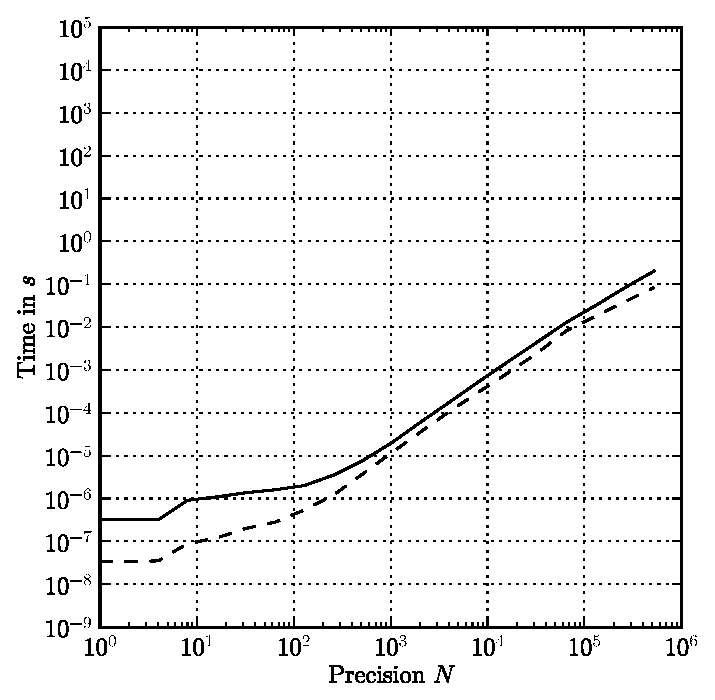
\includegraphics[width=0.84\textwidth]{bin/qp-mul.eps}
\end{minipage}
\begin{minipage}[t]{0.5\linewidth}
\centering
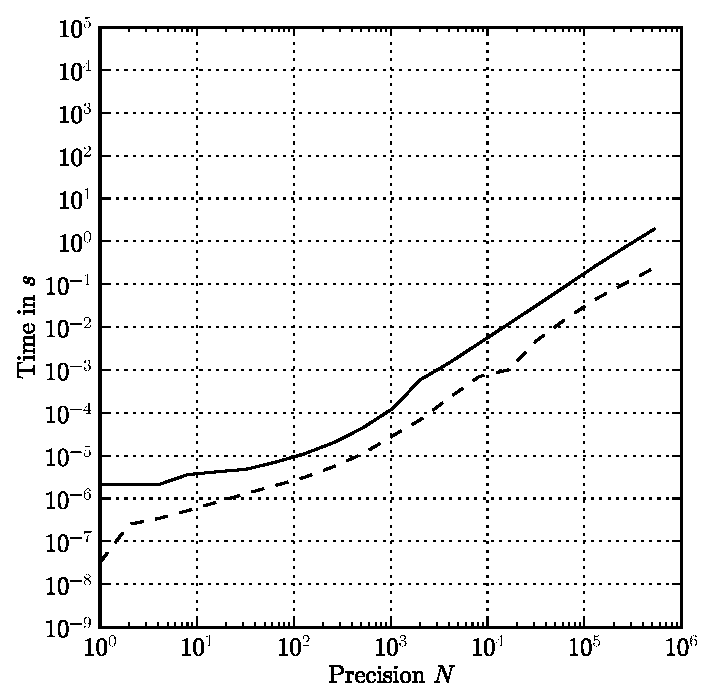
\includegraphics[width=0.84\textwidth]{bin/qp-inv.eps}
\end{minipage}\\

\begin{minipage}[t]{0.5\linewidth}
\centering
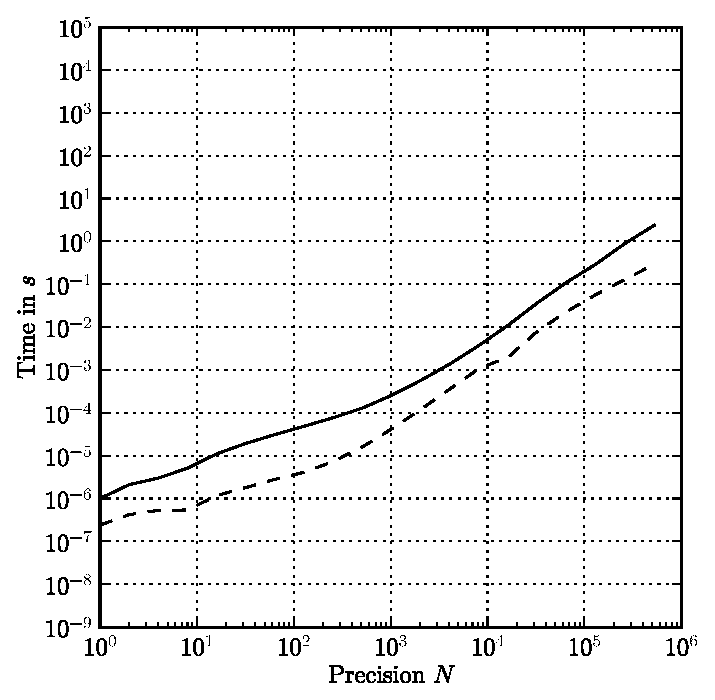
\includegraphics[width=0.84\textwidth]{bin/qp-sqrt.eps}
\end{minipage}
\begin{minipage}[t]{0.5\linewidth}
\centering
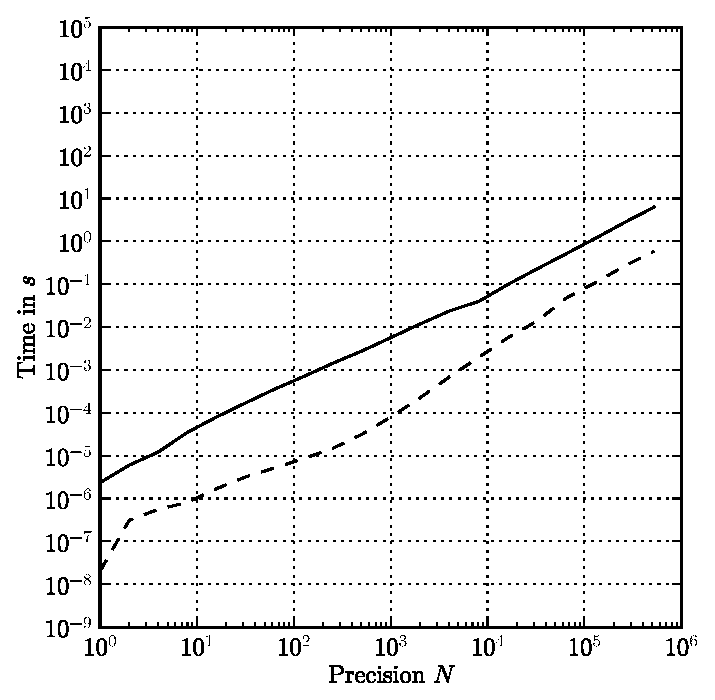
\includegraphics[width=0.84\textwidth]{bin/qp-teichmuller.eps}
\end{minipage}\\

\begin{minipage}[b]{0.5\linewidth}
\centering
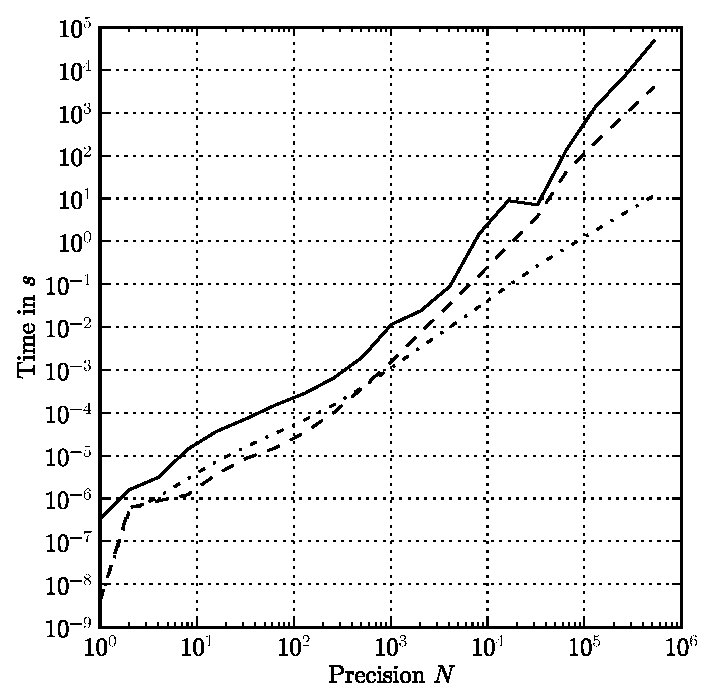
\includegraphics[width=0.84\textwidth]{bin/qp-exp.eps}
\end{minipage}
\begin{minipage}[b]{0.5\linewidth}
\centering
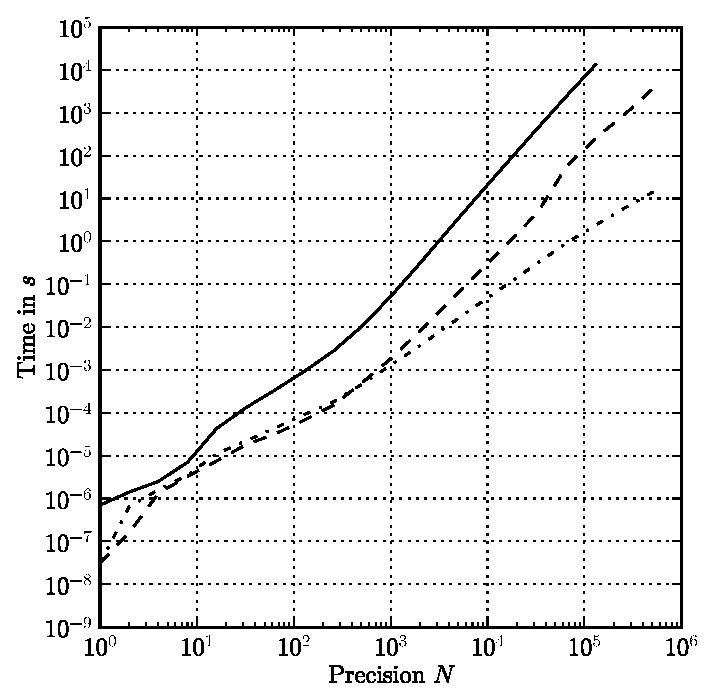
\includegraphics[width=0.84\textwidth]{bin/qp-log.eps}
\end{minipage}
\caption{From left to right, top to bottom, we compute 
$3^{3N} \times 5^{3N}$, $\bigl(3^{3N}\bigr)^{-1}$, $\sqrt{3^{6 N}}$, 
the Teichm\"uller lift of~$3$, $\exp\bigl(17 \times 3^{3N}\bigr)$, and 
$\log\bigl(1 + 17 \times 3^{3N}\bigr)$ modulo $17^N$.  The solid 
lines represent the routines in {\sc Magma}, the dashed and dotted 
lines the routines in {\sc FLINT}.}
\label{fig:timings-qp}
\end{figure}

\begin{figure}[ht]
\begin{minipage}[t]{0.5\linewidth}
\centering
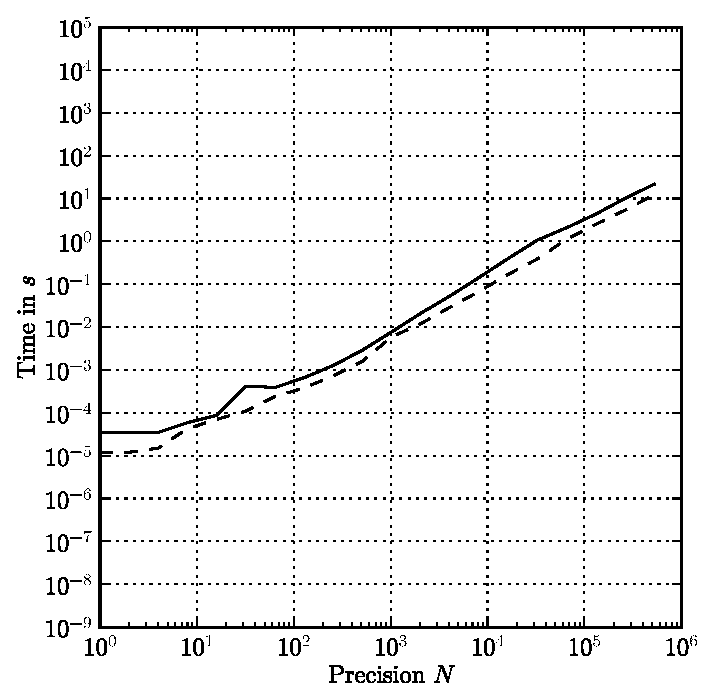
\includegraphics[width=0.84\textwidth]{bin/qq-mul.eps}
\end{minipage}
\begin{minipage}[t]{0.5\linewidth}
\centering
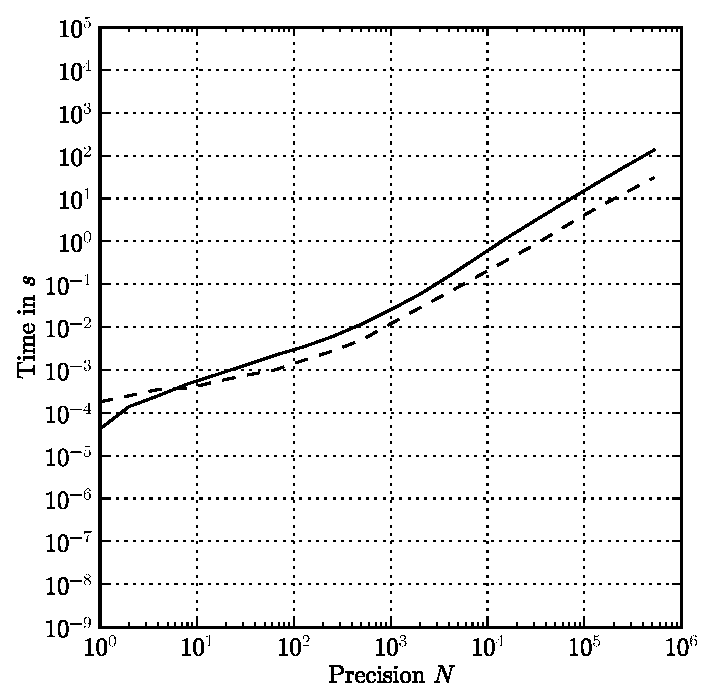
\includegraphics[width=0.84\textwidth]{bin/qq-inv.eps}
\end{minipage}\\

\begin{minipage}[t]{0.5\linewidth}
\centering
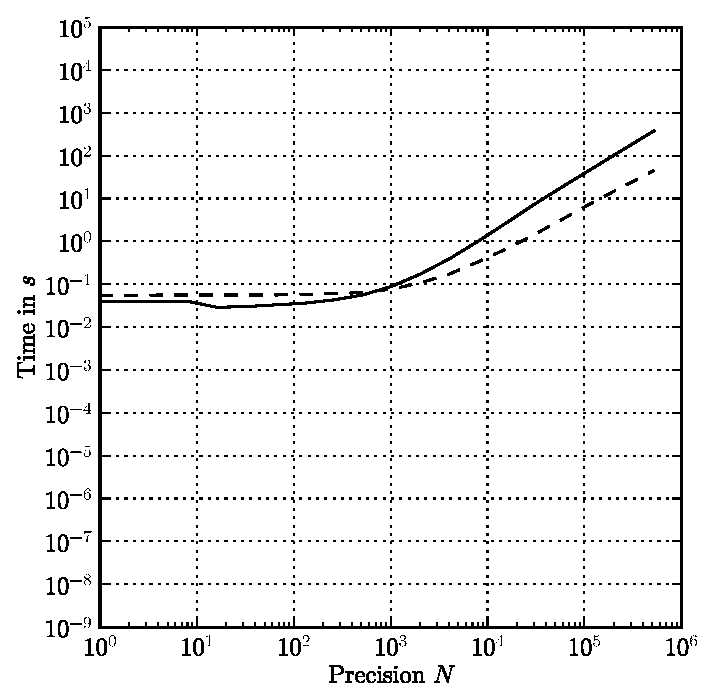
\includegraphics[width=0.84\textwidth]{bin/qq-sqrt.eps}
\end{minipage}
\begin{minipage}[t]{0.5\linewidth}
\centering
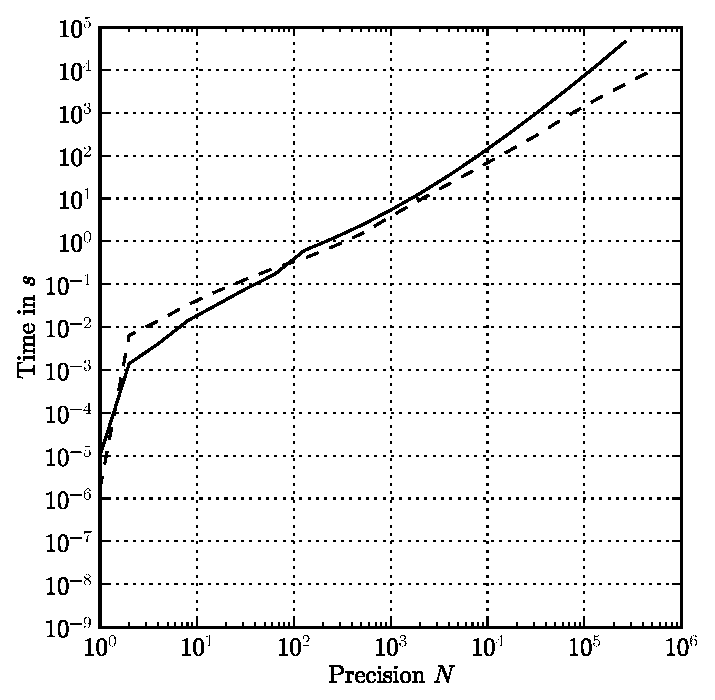
\includegraphics[width=0.84\textwidth]{bin/qq-teichmuller.eps}
\end{minipage}\\

\begin{minipage}[b]{0.5\linewidth}
\centering
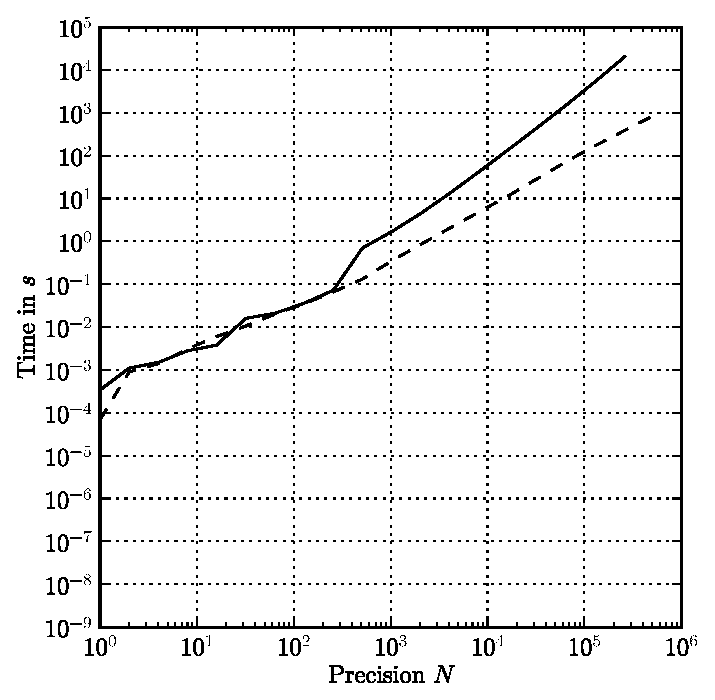
\includegraphics[width=0.84\textwidth]{bin/qq-frobenius.eps}
\end{minipage}
\begin{minipage}[b]{0.5\linewidth}
\centering
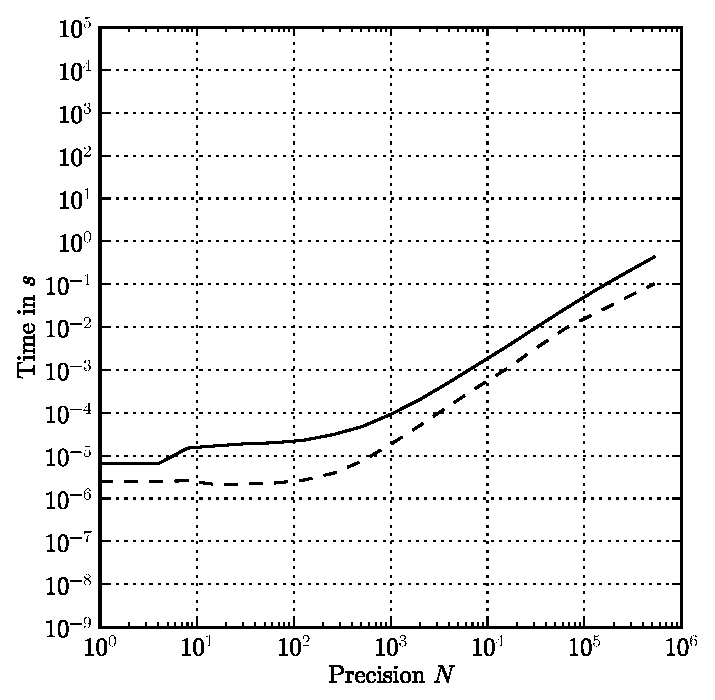
\includegraphics[width=0.84\textwidth]{bin/qq-trace.eps}
\end{minipage}
\caption{From left to right, top to bottom, we compute 
$a \times b$, $a^{-1}$ $\sqrt(a^2)$, the Teichm\"uller lift $c$, 
the Frobenius image of $a$, and the trace of $a$ in $\Z_{17^{97}}$ 
modulo $17^N$, where $a = \sum (3+i)^{3N} X^i$, $b = \sum (5+2i)^{3N} X^i$, 
and $c = \sum (3+i) X^i \bmod p$.
The solid lines represent the routines in {\sc Magma}, the dashed 
and dotted lines the routines in {\sc FLINT}.}
\label{fig:timings-qq1}
\end{figure}

\begin{figure}[ht]
\begin{minipage}[b]{0.5\linewidth}
\centering
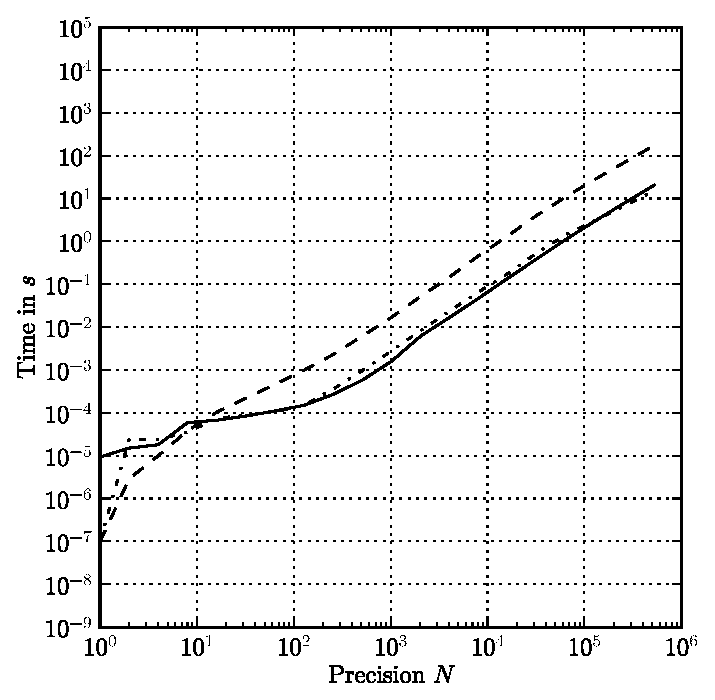
\includegraphics[width=0.84\textwidth]{bin/qq-norm_d5.eps}
\end{minipage}
\begin{minipage}[b]{0.5\linewidth}
\centering
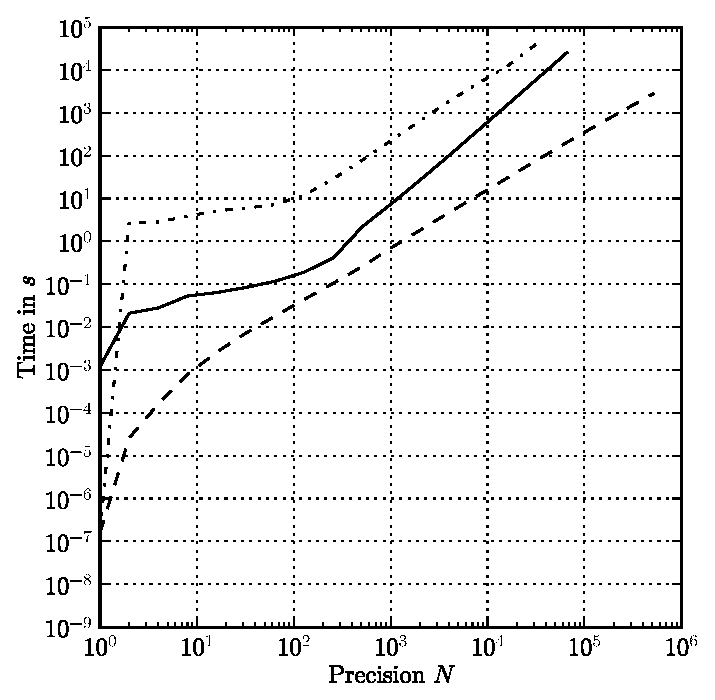
\includegraphics[width=0.84\textwidth]{bin/qq-norm_d97.eps}
\end{minipage}\\

\begin{minipage}[b]{0.5\linewidth}
\centering
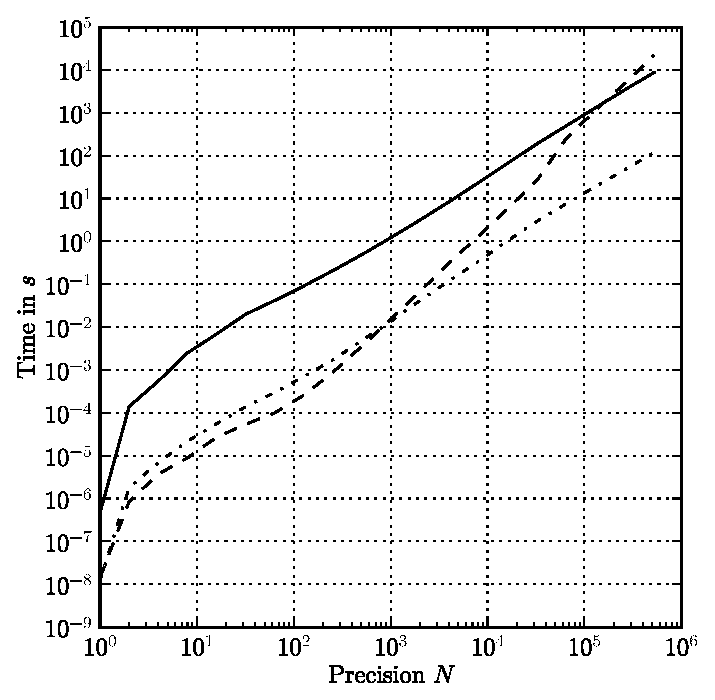
\includegraphics[width=0.84\textwidth]{bin/qq-exp.eps}
\end{minipage}
\begin{minipage}[b]{0.5\linewidth}
\centering
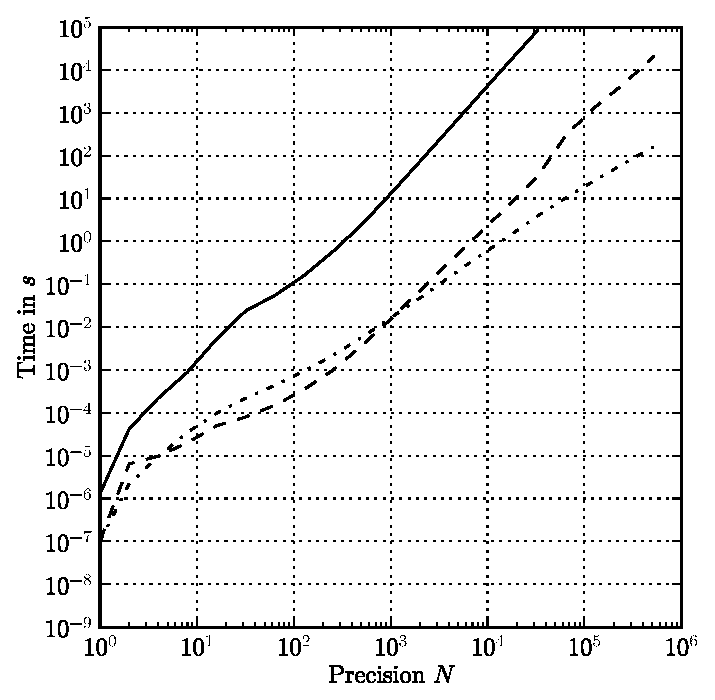
\includegraphics[width=0.84\textwidth]{bin/qq-log.eps}
\end{minipage}
\caption{From left to right, top to bottom, we compute the norm 
of $a$ in $\mathbf{Q}_{17^{5}}$ and $\mathbf{Q}_{17^{97}}$, and 
the exponential of $17 a$ and the logarithm of $1 + 17a$ in 
$\mathbf{Q}_{17^{97}}$, where $a = \sum (3+i)^{3N} X^i$.
The solid lines represent the routines in {\sc Magma}, the dashed 
and dotted lines the routines in {\sc FLINT}.}
\label{fig:timings-qq2}
\end{figure}

